%location/filename: tex/ch2.tex
%author: Anders Østevik
%Last edited: 03.05.2016
%#######--Chapter 2--#######
%Content:
%	hsmc-to-vldb pcb design
%	

\documentclass[main.tex]{subfiles}

\begin{document}

\chapter{HSMC-to-VLDB PCB Design} \label{chap:pcb}

In order to interface the radiation hard GBTx chip (see chapter \ref{chap:gbt}), a form of electrical connection between the \gls{fpga} and the \gls{vldb} is required. The \gls{vldb} board has twenty additional \acrshort{hdmi} female connectors which connects to \gls{lvds} transceivers for high-speed communication with the outside world. The \gls{fpga} board that is used for this thesis has two \gls{hsmc} connectors with port A containing pins that connects to \gls{lvds} transceivers. In addition, the \gls{vldb} connection also requires a radiation-hard optical link, i.e support for high-speed SFP fiber-optic cabling. For this, the \gls{hsmc} port A connector has also available pins that connects to \gls{xcvr} transceivers for transmission speeds up to $6.144\ \giga\bit\per\second$. The resulting \acrshort{pcb} has 10 individual \gls{hdmi} connector with each having one receiver and transmitter. Because of limited I/O, only one \gls{hdmi} contains a receiver reserved for input clock from the \gls{vldb}. This chapter explains the process of making such a \gls{pcb}, from the discussion of different design approaches to the theory behind designing a high speed \gls{pcb}. \\

\section{Design Discussion}

The design discussion and planning of the \gls{pcb} was done together with Ph. D. Arild Velure.\\

The initial plan was to design a \gls{pcb} with a male \gls{sfp}-contact in one end connected with two \gls{hdmi} connectors, one on each side of the \gls{pcb}, making an adapter that can be plugged directly into the \gls{sfp}-connectors on the \gls{sfp}-board with \gls{hdmi} cables to the \gls{vldb}. This design was quickly scratched as there was no loose male \gls{sfp} connectors available on the marked, only female. The design plan was then changed to use only one \gls{pcb} board with female \glspl{sfp}-connectors on one side, wired to \gls{hdmi}-connectors on the other side, acting as a middle joint between the \gls{sfp}-board and the \gls{vldb} with \gls{sfp}- and \gls{hdmi}-cables connecting the three boards together. \\


The end result was a design that could be directly mounted on the \gls{fpga} through the \gls{hsmc} connector. By copying one of the \gls{sfp}-to-\gls{hsmc} connections from the original \gls{sfp}-board design files (the one concerning the \gls{xcvr}-protocol, see \cite{sfp_schem}), we found that we could remove the \gls{sfp}-board completely from the connection chain and eliminate the resulting need for electrical \gls{sfp}-cables. This would also remove the middle joint in the chain, reducing complexity and lowering the chance of signal reflections. %The resulting design was a board connected to the \gls{fpga} via the \gls{hsmc}-connector, with \gls{lvds}-signals running to ten \gls{hdmi} connectors and \gls{xcvr}-signals running to one \gls{sfp}-connector for fiber-optic communication.

\begin{figure}[ht] % H(strictly put HERE > h!)
% h(here), !(force), t(top), b(bottom), p(on extra page)
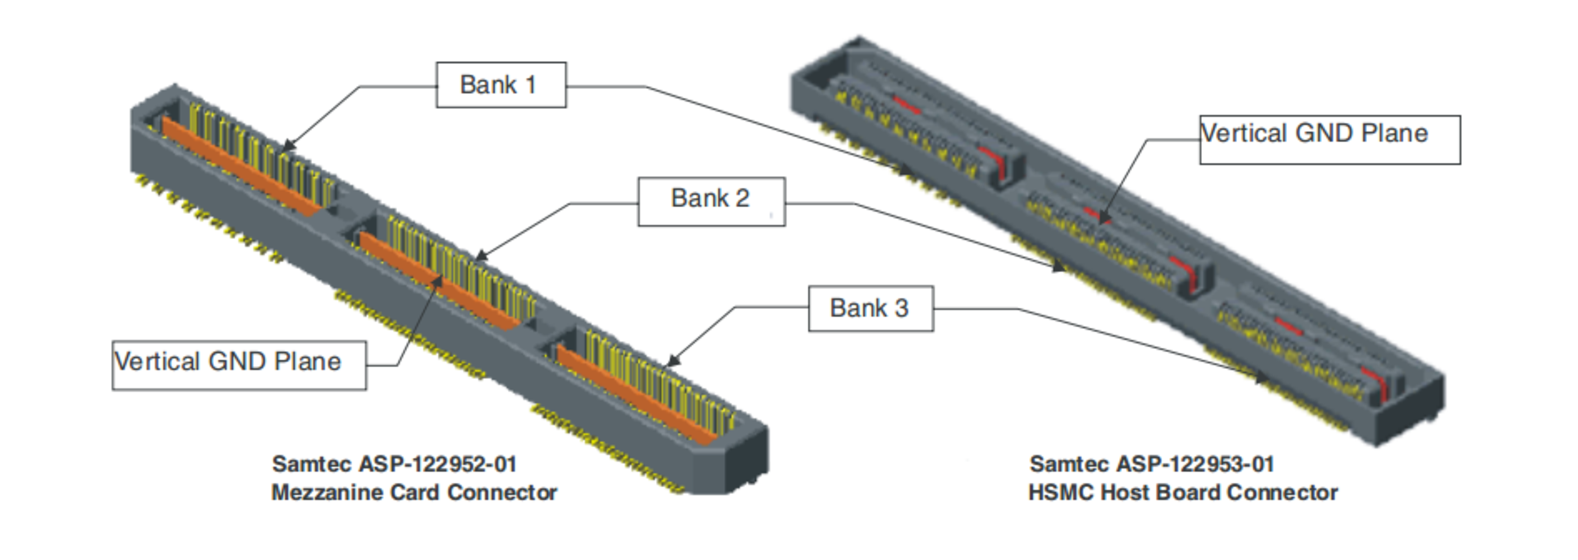
\includegraphics[width=\linewidth]{../img/HSMC_52_53_hsmcspec}  \\[0.1 cm]
\caption{Male (ASP-122952) and female (ASP-122953) HSMC-connectors. The male type is to be connected at the bottom of the HSMC-to-VLDB \gls{pcb} \cite[Figure 2-1]{altera_hsmc09}.}
\label{fig:hsmc}
\end{figure}

\section{High Speed PCB Design}

When transmitting signals through a conductor at high frequencies, the conductor no longer acts as an ideal wire. The signal voltage stops acting instantaneous across the conducting path, and factors like impedance mismatch and reflections becomes important for the quality of the signal to remain the same through the whole transmission. This section gives a brief explanation of high frequency signal behavior and the compensation methods that was practiced during the design of the \gls{hsmc}-to-\gls{vldb} \gls{pcb}.

\subsection{Transmission Lines}

When signal rise/fall times becomes comparable with the propagation delay of the conductor, the signal no longer acts instantaneous. The conductor becomes what is known as a transmission line, with the signals voltage and current acting like waves propagation through the conductor. 
The general rule for determining if a signal is propagating along a transmission line is when the rise/fall time of the signal is less than 1/4 of the signal period, so that the high and low states are recognizable \cite{weste11}.

For an \gls{lvds}-protocol, with signal speeds reaching up to $3.125\ \giga\bit\per\second$, the trace becomes a transmission line if the signal propagation time along the trace is less than 1/4 of the signal period, i.e $80\pico\second$. 

The propagation velocity of a signal is given by:

\begin{equation}
%\[
    v = \frac{c}{\sqrt{\epsilon_r}}
%\]
\end{equation}

, where $\epsilon_r$ is the dielectric constant of the epoxy material FR4, often used as a material to separate the copper layers on the \glspl{pcb}. $\epsilon_r$ has a value of around $4.05$ @ $3\ \giga\hertz$ \cite{polar15}.
A signal thus propagates through the conductor at a velocity of approximately $15\ \milli\meter/\nano\second$ \cite[example 13.7]{weste11}.

Thus, by assuming a constant transmitting frequency of $3.125\ \giga\bit\per\second$, a conductor becomes a transmission line if the length of the conductor stretches longer than $12\ \milli\meter$ between transmitter and receiver. This short length is very difficult to avoid when designing a \gls{pcb} with microstrip traces running from one connector out to eleven other connectors. The traces on the HSMC-to-VLDB \gls{pcb} are therefore considered as transmission lines. 

\subsection{Reflections and Characteristic Impedance}

Since the signals no longer acts instantaneous, the transmitter can not see what is connected at the receiving end at the time it sends a pulse down the conducting channel. All it sees is the channel impedance, called the characteristic impedance, $Z_0$, of the channel \cite{weste11}.

The type of trace that is used in the \gls{hsmc}-to-\gls{vldb} \gls{pcb} design is called a microstrip, which is when the signal traces run along traces on the outer layers of the \gls{pcb} with the ground plane on the layer underneath. 

A microstrip has a characteristic impedance that is given by:

\begin{equation}
    Z_0 = \frac{60}{\sqrt{0.475\epsilon_r + 0.67}} \times \ln{\frac{4h}{0.67(0.8w + t)}}
\end{equation}

, where $\epsilon_r$ is the dielectric constant, h is the height of the microstrip seen from the ground plane, i.e the thickness of the FR4 layer, w is the width of the microstrip, and t is the thickness of the copper \cite{weste11}.

It is important to match the impedance of the trace to that of the load impedance at the receiving end, or vice versa. With these being different, the energy of the signal cannot be fully absorbed at the receiving end, resulting in a partly reflection of the signal wave back to the transmitter. The ratio of the wave reflected back is given by:

\begin{equation}
\Gamma = \frac{Z_L - Z_0}{Z_L + Z_0}	
\end{equation}

, where $Z_L$ is the load impedance and $Z_0$ is the characteristic impedance.

Ideally the $Z_L$ and $Z_0$ should be equal to avoid reflections. Impedance mismatch can cause waste of signal energy and interference with other signal pulses being transmitted through the channel \cite{weste11}. \\

When looking at the datasheet for cables with differential signals, such as HDMI-cables, it is often supplied a differential impedance between the cables instead of a characteristic impedance for each cable. Knowing the characteristic impedance, it is possible to calculate the corresponding differential impedance between two microstrip traces (or vice versa):

\begin{equation}
    Z_{diff} = 2 \times Z_0 [1 - 0.48 e^{(-0.96 \times \frac{s}{h})}]
\end{equation}

, where $Z_0$ is the characteristic impedance of the individual microstrips (assuming they are equal and have the same length), s is the spacing between the microstrips and h is the same as in the equation above \cite{douglas98}.

\definecolor{FR4}{HTML}{20B356}
\definecolor{COPPER}{HTML}{FFA500}

\begin{figure}[H]
  \begin{subfigure}[t]{0.45\textwidth}
    \centering
    %Microstrip single-ended
    \resizebox{\linewidth}{!}{
    \begin{tikzpicture}
        
      %Ground Plane
      \draw[yslant=0,fill=COPPER,opacity=1] (0,-1.0) rectangle (4,-0.8);  %Front
      \draw[yslant=0.5, fill=COPPER,opacity=1] (4,-2.8) rectangle (6,-3); %Side
      %\draw[yslant=0.5,xslant=-2] (0.4,0.2) rectangle (2.4,-1.8);           %Top

      %FR4 Plane
      \draw[yslant=0.0, fill=FR4,opacity=1] (0,-0.8) rectangle (4,0.2);                %Front
      \draw[yslant=0.5, fill=FR4,opacity=1] (4,-2.8) rectangle (6,-1.8);               %Side
      \draw[yslant=0.5,xslant=-2, fill=FR4!90,opacity=1] (0.4,0.2) rectangle (2.4,-1.8);  %Top

       %Trace
      \draw[yslant=0,fill=COPPER] (1.45,0.2) rectangle (2.45,0.38);                   %Front
      \draw[yslant=0.5,fill=COPPER] (2.44,-0.85) rectangle (4.45,-1.02);            %Side
      \draw[yslant=0.5,xslant=-2, fill=COPPER!80] (0.75,-0.85) rectangle (2.74,-0.35); %Top

      \draw[<->] (0.4,-0.8) -- (0.4,0.2) node [midway,fill=FR4] {h};
      \draw[|<->|] (1.45,-0.2) -- (2.45,-0.2) node [midway,fill=FR4] {w};
    
       \draw[] (-0.4,0.38) -- (1.6,1.38) node [midway, fill=white] {l};

      \draw[|<->|] (1.2,0.195) -- (1.2,0.38) node [left] {t};

    \end{tikzpicture}
    }
    \caption{Single-ended.}
  \end{subfigure}
  ~
 %Microstrip differential
  \begin{subfigure}[t]{0.45\textwidth}
  \centering
    \resizebox{\linewidth}{!}{
  \begin{tikzpicture}
      
    %Ground Plane
    \draw[yslant=0,fill=COPPER,opacity=1] (0,-1.0) rectangle (4,-0.8);  %Front
    \draw[yslant=0.5, fill=COPPER,opacity=1] (4,-2.8) rectangle (6,-3); %Side

    %FR4 Plane
    \draw[yslant=0.0, fill=FR4,opacity=1] (0,-0.8) rectangle (4,0.2);                %Front
    \draw[yslant=0.5, fill=FR4,opacity=1] (4,-2.8) rectangle (6,-1.8);               %Side
    \draw[yslant=0.5,xslant=-2, fill=FR4!90,opacity=1] (0.4,0.2) rectangle (2.4,-1.8);  %Top

    %Trace#1
    \draw[yslant=0,fill=COPPER] (0.45,0.2) rectangle (1.45,0.38);                   %Front
    \draw[yslant=0.5,fill=COPPER] (1.45,-0.35) rectangle (3.45,-0.53);            %Side
    \draw[yslant=0.5,xslant=-2, fill=COPPER!80] (0.75,0.15) rectangle (2.74,-0.35); %Top

    %Trace#2
    \draw[yslant=0,fill=COPPER] (2.45,0.2) rectangle (3.45,0.38);                   %Front
    \draw[yslant=0.5,fill=COPPER] (3.45,-1.35) rectangle (5.45,-1.53);            %Side
   \draw[yslant=0.5,xslant=-2, fill=COPPER!80] (0.75,-0.85) rectangle (2.74,-1.35); %Top

    \draw[<->] (0.25,-0.8) -- (0.25,0.2) node [midway,fill=FR4] {h};

    \draw[|<->|] (0.45,-0.2) -- (1.45,-0.2) node [midway,fill=FR4] {w};
    \draw[<->] (1.45,-0.2) -- (2.45,-0.2) node [midway,fill=FR4] {s};
    \draw[|<->|] (2.45,-0.2) -- (3.45,-0.2) node [midway,fill=FR4] {w};
    
    \draw[|<->|] (2.1,0.19) -- (2.1,0.38) node [right] {t};
    
    \draw[] (-0.4,0.38) -- (1.6,1.38) node [midway, fill=white] {l};

  \end{tikzpicture}
  }
     \caption{Differential.}
  \end{subfigure}
      \caption{Microstrip, cross-section. The microstrip is the copper trace(s) on top, followed by a dielectric layer and a ground plane. h is the thickness of the dielectric, t is the copper thickness, l is the microstrip length, and w is the copper width. s is the spacing between the differential strips.}
    \label{fig:microstrip}
\end{figure}

\subsection{Routing}

As mentioned in section~\ref{subsec:diffsig}, differential signals have noise advantages over single ended signals. This is the case only if the pairs have \textit{equal} path lengths and the individual wires in each pair are routed as close to one another as possible. In addition, to keep crosstalk to its minimum, individual pairs has to be routed a distance away from other wires (In reality, this only becomes a problem when dealing with wiring in the micro-scale domain). Twisting the individual wires in each pair to some extent will also contribute to common noise rejection \cite{weste11}.
This was taken into consideration when routing the \gls{pcb}. 

The individual wires in each pair was kept as close as possible, with a space constraint (See table \ref{tab:Xsect1}) according to the required differential impedance $Z_{diff}$ of approximately $100\ \ohm$ (See equation \ref{eq:zdiff}). When routing, twisting the wires (where possible) was achieved by purposely making the wires overlap at the viases. After routing the wires, attempts were made to separate the pairs a distance from one another, but this was not a critical stage.

\section{PCB Design Parameters}

The \gls{pcb} schematic was designed using \textit{Orcad Capture CIS} and the layout using \textit{Orcad \gls{pcb} Editor}, with design parameters meeting \textit{Elprint's} capabilities \cite{elprint15}. The \gls{pcb} layout was then exported into \textit{Gerber-files} and imported into \textit{Macaos} for further manufacture specification and validation. The \gls{pcb} was then ordered from Elprint. \\% and arrived in office 21/12/2015.

To avoid signal reflections, the \gls{pcb} needed a characteristic impedance matching that of the cables and termination, in this case a single wire impedance of $50\ \ohm$, and a differential impedance of $100\ \ohm$. This was derived from the fact that the \gls{hdmi}-cables were specified to have a differential impedance of approximately $100\ \ohm$, and that the individual transceiver lines from the \gls{fpga} has a characteristic impedance of $50\ \ohm$, with a selectable termination resistance at the receiving end of $100\ \ohm$, connected between the lines.

The \gls{pcb} was chosen to be four layers, with signals running on the top and bottom copper layers, and the two middle planes for voltages and ground respectively.

For thicknesses of the different \gls{pcb} copper layers and the FR4 in between, Elprint has a set of predefined \textit{stack-ups} available in Macaos. It is possible to define custom stack-ups as well, but this will result in a more costly \gls{pcb}. The $4036$ pre-defined stack-up has a copper thickness of $18\ \micro\meter$ on the two outer layers following an FR4 thickness of $65\ \micro\meter$ between the outer layers and the power planes, with the power planes having a thickness of $35\ \micro\meter$. Between the power planes is another FR4 layer with a thickness of $1.4 \milli\meter$ making the total \gls{pcb} thickness of a standard $1.6 \milli\meter$. With a mircostrip width of $100\ \micro\meter$, the formula for characteristic impedance yields:

\begin{equation}
Z_0 = \frac{60}{\sqrt{(0.475 \times 4.05) + 0.67}}\ln{3.96}
\end{equation}

, which gives a characteristic impedance $Z_0$ of $51.3\ \ohm$ @ $3\ \giga\hertz$. 

With a $300\ \micro\meter$ spacing between the differential traces, the formula for differential impedance yields:

\begin{equation}
    Z_{diff} = 2 \times 51.3\ \ohm [1 - 0.48 e^{(-0.96 \times \frac{300}{65})}]
  \label{eq:zdiff}
\end{equation}

, which gives a differential impedance $Z_{diff}$ of $102\ \ohm$ @ $3\ \giga\hertz$.\\

Table \ref{tab:Xsect1} shows data extracted from Orcad PCB Editor, which has a built-in impedance calculator that yields similar results as shown above:

\begin{table} [H]
\begin{center}
    \begin{tabular}{ l | l | l | l | l | l | l | l | l }
    \hline
     & Layer & Type & t $[\micro\meter]$ & $\epsilon_r$ & w $[\micro\meter]$  & $Z_0 [\ohm]$ & Spacing $[\micro\meter]$  & $Z_{diff} [\ohm]$ \\ 
     \hline
    1 	  & Surface & Air 		 & 		& 1 	 & 	   & 					& 	  & \\ \hline
    2 	  & Top 	& Conductor  & 18 	&        & 100 & $51.3$             & 300 & 102\\ \hline
    3 	  &  		& Dielectric & 65 	& $4.05$ & 	   & 					& 	  & \\ \hline
    4 	  & Voltage & Plane 	 & 35 	&        & 	   & 					& 	  & \\ \hline
    5 	  &  		& Dielectric & 1400 & $4.05$ & 	   &					&	  & \\ \hline
    6 	  & Gnd 	& Plane 	 & 35 	&        & 	   & 					& 	  & \\ \hline
    7 	  &  		& Dielectric & 65 	& $4.05$ &     & 					& 	  & \\ \hline
    8 	  & Bottom 	& Conductor  & 18 	&        & 100 & $51.3$             & 300 & 102\\ \hline
    9 	  & Surface & Air 		 & 	  	& 1 	 & 	   & 					& 	  & \\ \hline
    \end{tabular}
     \caption{The layers of the PCB and their traits, where t is the layer thickness and w is the width of the trace. The PCB has an overall thickness of $1.6\ \milli\meter$}
	\label{tab:Xsect1}
\end{center}
\end{table}

%\section{Further specification and ordering}

\section{Pads and Footprints}

All pads and footprints were custom made using \textit{Cadence Pad Designer}, with dimensions collected from datasheets of the different components. The only excepting was for the \gls{hsmc} footprint and pads, which were acquired from the manufacturer. The pads were dimensioned a bit longer than the actual pins, making it a bit easier to make contact with the soldering iron when soldering by hand.

\section{Soldering Process}

All the components on the \gls{pcb} was soldered by hand, with the exception of the ground pads underneath the \gls{hsmc}, which had to be soldered using solder paste and a solder oven. The solder paste, which is a lead contained paste of type \textit{EFD SolderPlus 221 RMA}, was ordered from \url{www.krepro.no} in late January 2016.

\subsection{Soldering the Ground Pads Underneath the HSMC Contact}

The \gls{hsmc}-connector has several ground pads underneath the connector itself, making it impossible to reach when soldering by hand. The solution to this use a solder oven with solder paste on the pads. The solder paste was applied on the pads with the help of the dispenser module on the \textit{Martin Rework Station}, which was available in the lab. The dispenser module forces the solder paste out of the syringe using pressurized air. By pressing a foot pedal connected to the dispenser, you apply a controlled air pulse that pushes on the piston of the solder paste syringe. The force of the air pulse can be adjusted using the dispenser \gls{gui}. For the ground pads, a force of $2.50~ccm$ was suitable.

The solder oven that was used had the option to set up a \textit{Ramp-Soak-Spike} type thermal profile. Samtec, the manufacturer for the \gls{hsmc} contact, recommends a maximum peak temperature of no more than $260~\degree C$ with no more than 30 seconds above $255\degree C$. The thermal profile setup is based on the profile recommended by EFD, the manufacturer for the particular solder paste used (see figure \ref{fig:krepro}). After some trial and error with a dummy-PCB, the oven was set to a activation temperature of $150\degree C$ for $60~seconds$, and then a reflow temperature of $220\degree C$ with a climb-time of $120~seconds$. 

\begin{figure}[H] % H(strictly put HERE > h!)
% h(here), !(force), t(top), b(bottom), p(on extra page)
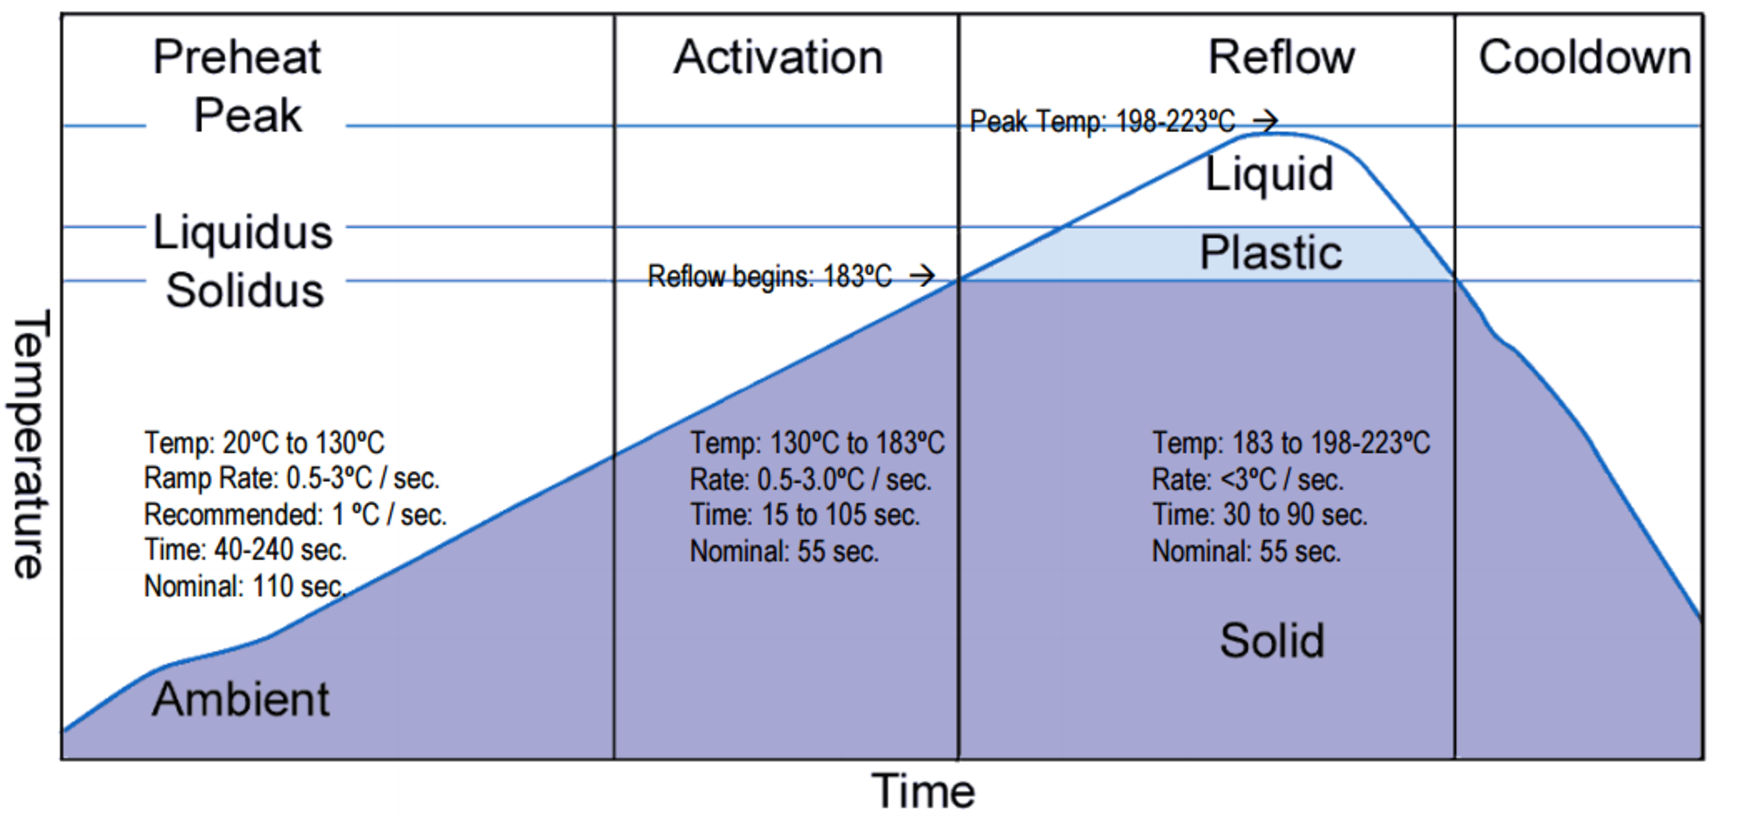
\includegraphics[width=0.8\linewidth]{../img/temp_prof}  \\[0.1 cm]
\caption{EFD reflow thermal profile recommendations \cite{krepro_reflow}.}
\label{fig:krepro}
\end{figure}

The finished PCB is shown in figure \ref{fig:pcb_1}. The \gls{hsmc} contact is located at the bottom of the \gls{pcb}.

\begin{figure}[H] % H(strictly put HERE > h!)
% h(here), !(force), t(top), b(bottom), p(on extra page)
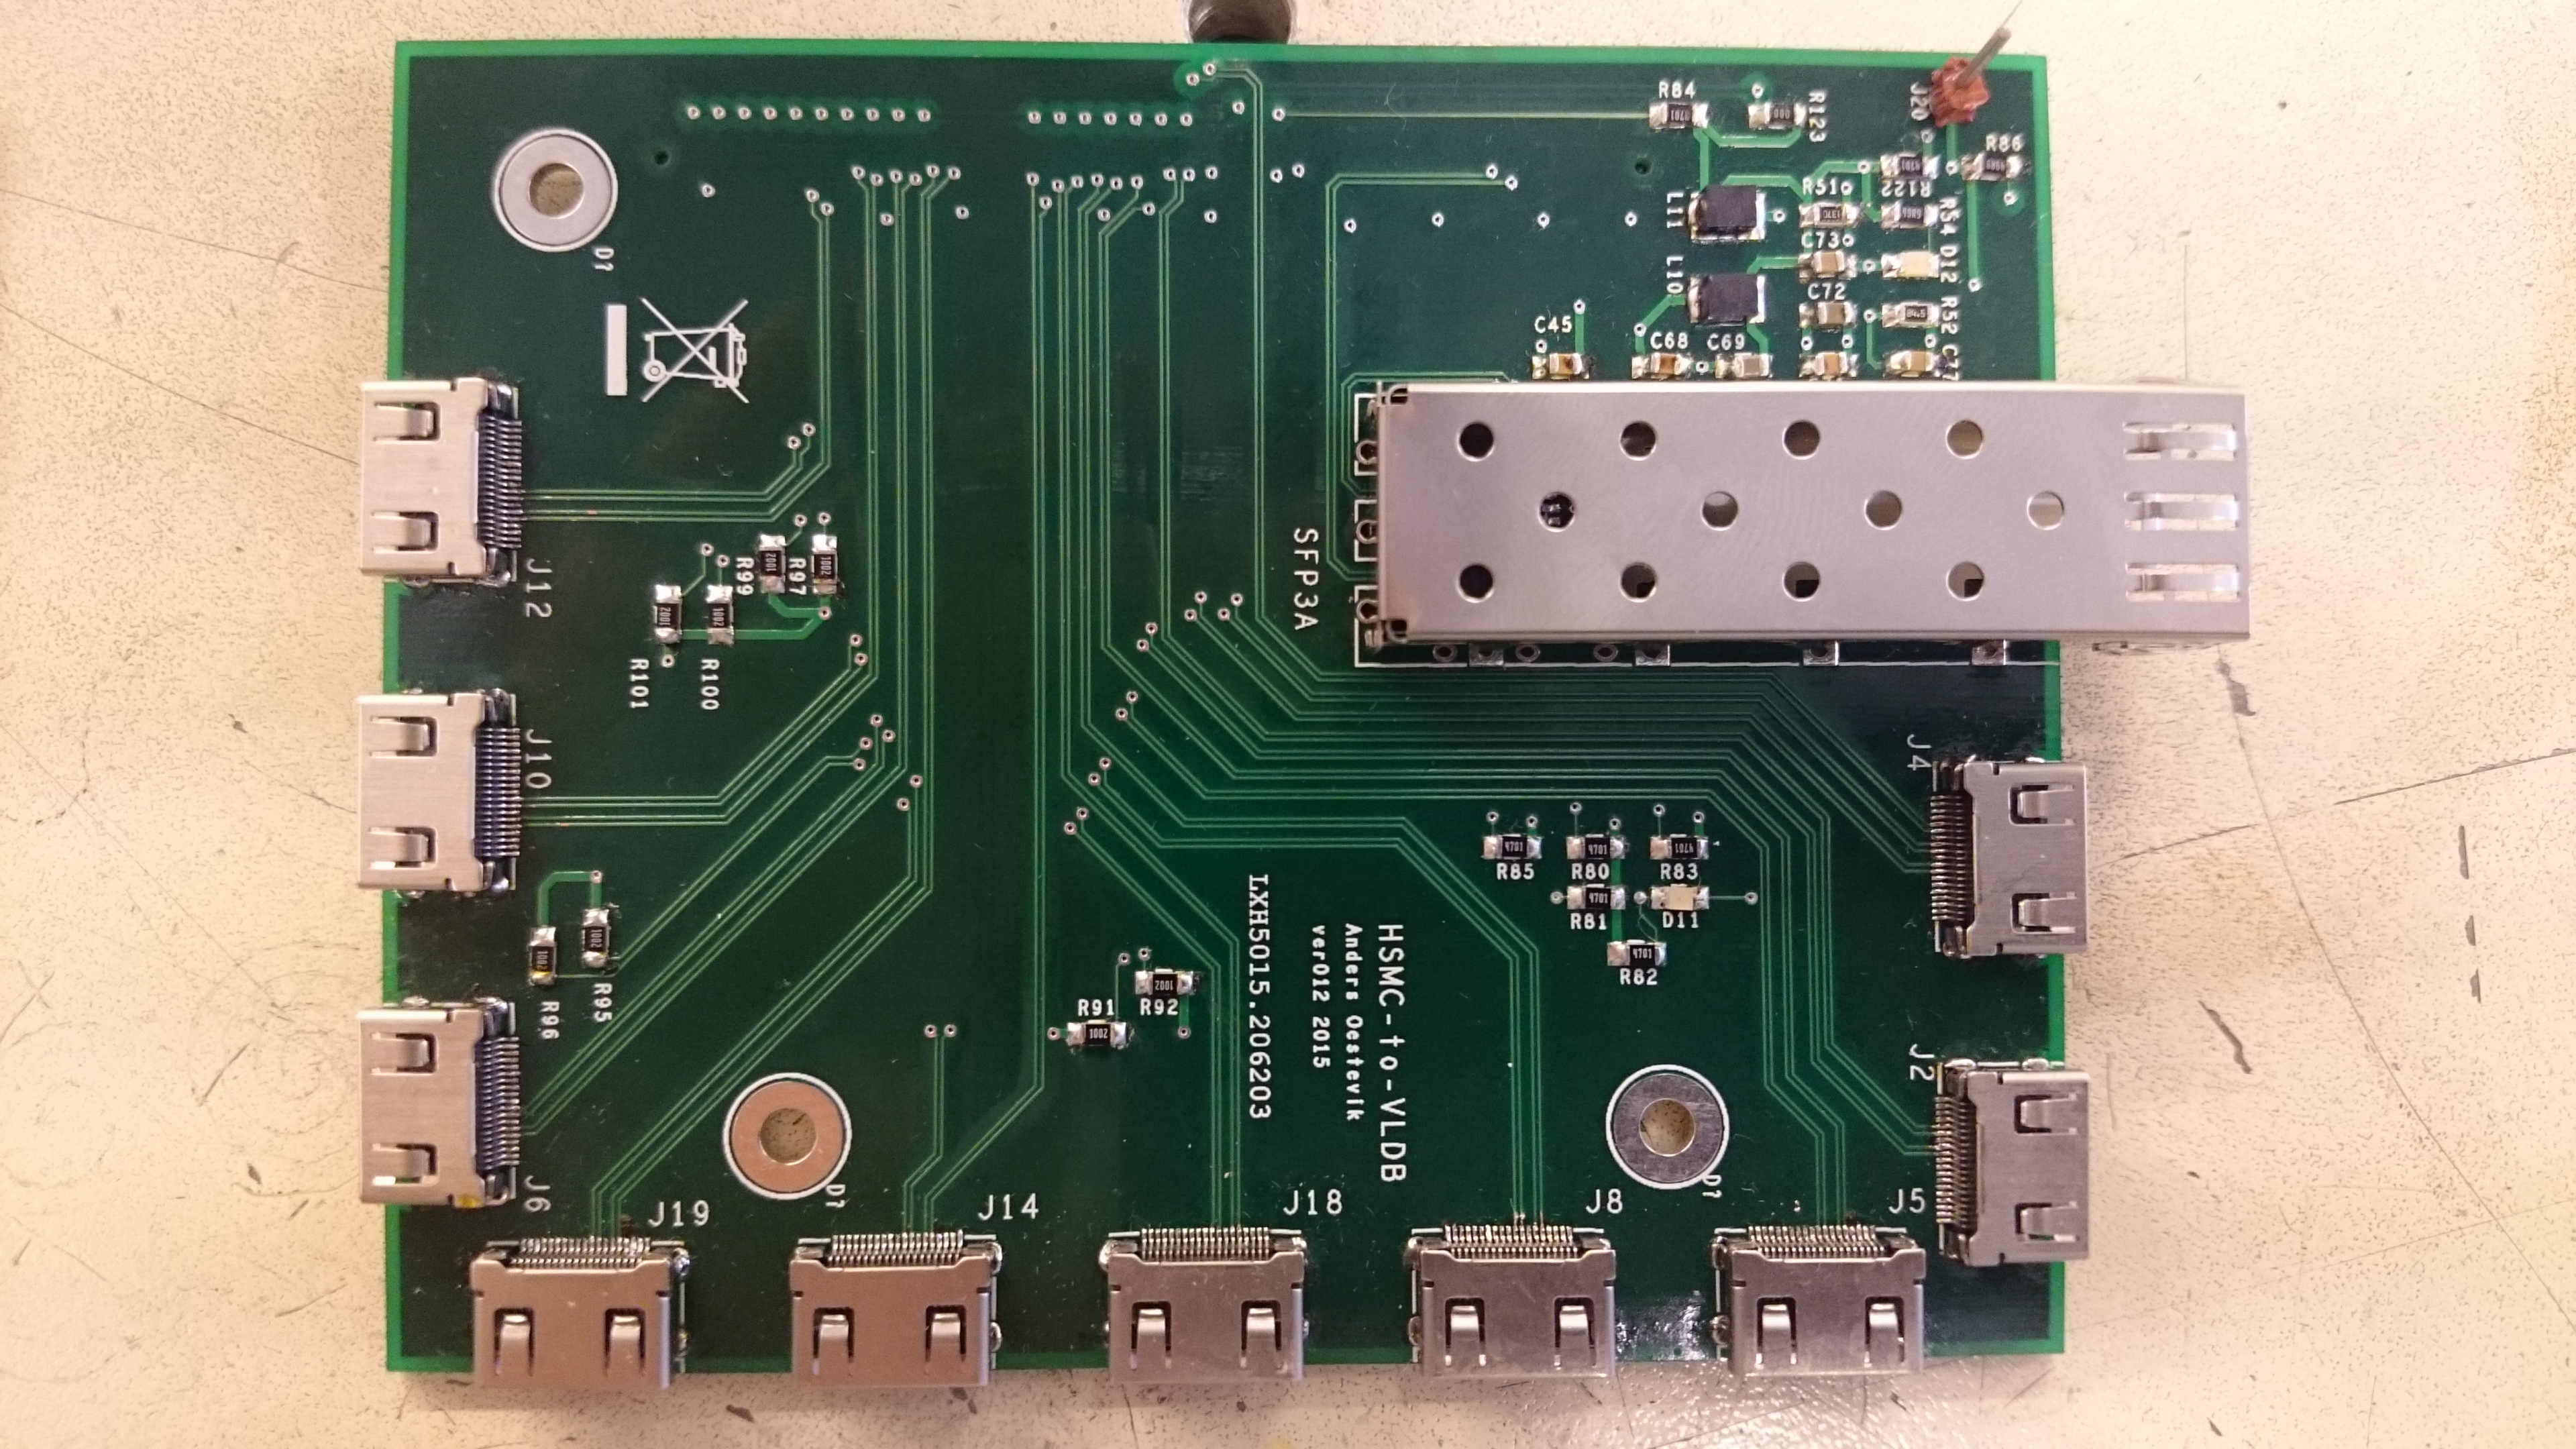
\includegraphics[width=0.8\linewidth, trim={15cm 0 15cm 0},clip]{../img/pcb_1.JPG}  \\[0.1 cm]
\caption{HDMI-to-VLDB PCB with components soldered on.}
\label{fig:pcb_1}
\end{figure}

\section{PCB Faults and Compensations}

During the process of hand soldering, it was discovered that the \gls{hsmc} pads were dimensioned for the purpose of reflow soldering using a solder oven. This meant that the pads were dimensioned to match exactly that of the pins, making it very difficult to solder by hand. With 160 individual pins to be soldered to the \gls{pcb} board, this resulted in a time-consuming work with a lot of effort trying to keep the pins from shorting. To ease the soldering process of the \gls{hsmc}, the pads should be dimensioned a bit longer.

After receiving the \glspl{pcb}, further inspection revealed that all viases had missing solder mask. This exposes the metal of the vias to the surface of the \gls{pcb} and can possibly cause connection shorts between the viases and the pads and/or metallic casings when soldering. The reason for the viases not to have a solder mask is because it was missing in the pad file. A solution to fix this in a future \gls{pcb} print would obviously be to include a solder mask in the pad file.
With the current \gls{pcb} print, however, a temporary solution would be to apply thin \textit{kapton tape} where most critical.\\

The exposed viases was later shown not to be as critical as first thought, due to the following points:\\

\begin{itemize}\setlength{\itemsep}{10pt}
\item The viases that are exposed underneath the \gls{hdmi} casings are in fact connected to ground, making the possible shorts between the viases and the already ground connected casing not a critical problem.
\item The exposed viases underneath the \gls{hsmc}-connector could potentially connect to the ground pads when applying solder paste to the pads. This was avoided by carefully applying  a thin line of solder paste in the middle of the ground pads. This prevented the solder paste to float over to the neighboring viases when melting it in the oven. A possible drawback to this would be bad connection between the ground pads and the \gls{hsmc}-connector, but a quick check using a multimeter proved that the \gls{hsmc} was indeed connected to all the ground pads.\\
\end{itemize}

In fact, when testing the \gls{pcb}, the exposure of viases on the transmitter and receiver lines revealed to be quite useful probe points when using an oscilloscope to measure the signal integrity. Due to the lack of extra added probe points, measuring signals at the \gls{pcb} viases became the most convenient way of directly measuring the signals on the transmitter and receiver lines (see subsection below). A lesson until next \gls{pcb}-prototype is to include easily accessible probe points on lines that are relevant for oscilloscope measurement.\\

\begin{figure} % H(strictly put HERE > h!)
% h(here), !(force), t(top), b(bottom), p(on extra page)
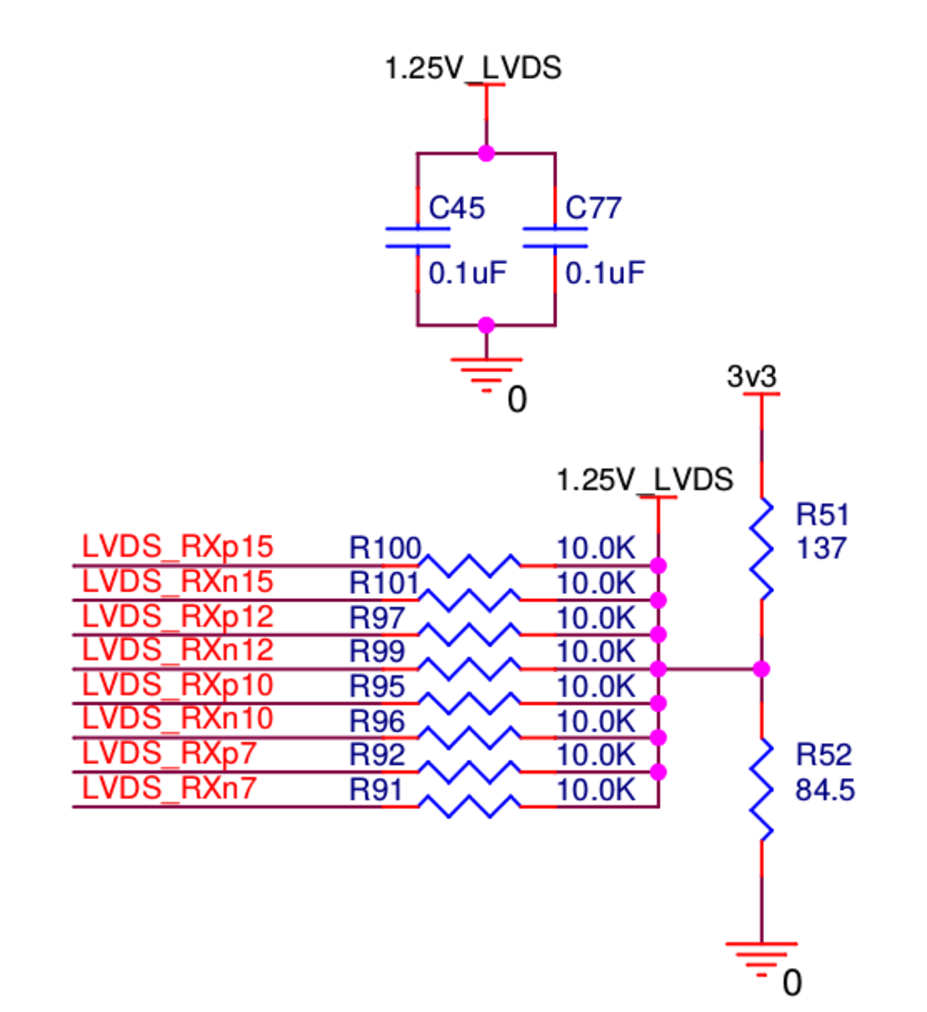
\includegraphics[width = 7 cm]{../img/pullups}  \\[0.1 cm]
\caption{Pull-up resistors on some of the receiver lines.}
\label{fig:pullups}
\end{figure}

On the current version of the \gls{pcb}, some of the receiver lines includes a $10~\kilo\ohm$ pull-up resistor (R91, R92, R95, R96, R97, R99, R100 and R101 in the schematic). The reason why these are included could possibly be due to a misinterpretation of the \gls{sfp}-schematic in which the design of the \gls{pcb} was based on. This is concluded because two of the pull-up resistors (R100 and R101 in the schematic) are connected to receiver signals that are only used in the \gls{sfp}-design, but not in this design. The pull-up resistor pads were therefore not soldered on the board, and the lines were left open.


%Later discussions with Arild revealed that the transmitters on the GBT-VLDB did not have voltage pull-ups, which is necessary for the \gls{lvds}-signals. The current \gls{pcb} will therefore not work properly with the GBT-VLDB card. Later versions of the \gls{pcb} should therefore contain resistors pulling up to $1.25 \volt$ on the receiver lines in order for it to work.

\end{document}